% Components of the reachability graph for a fixed arc step.
\documentclass[tikz,border=8pt]{standalone}
\usepackage{amsmath,amssymb}
\usetikzlibrary{arrows.meta}
\begin{document}
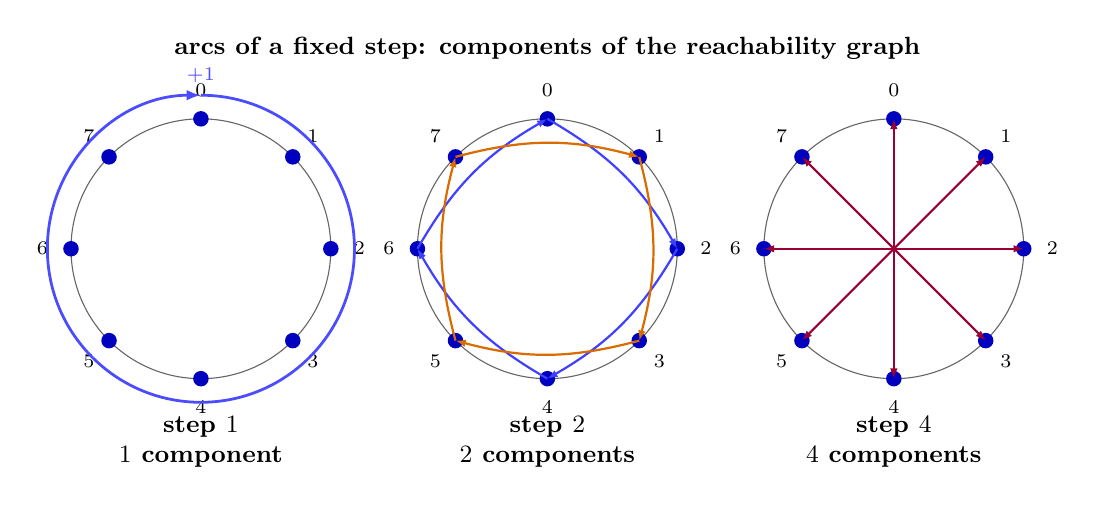
\begin{tikzpicture}[
  dot/.style={fill=blue!75!black, circle, inner sep=0pt},
  arr/.style={-{Latex[length=1.3mm]}, line width=0.8pt},
  darr/.style={{Latex[length=1.3mm]}-{Latex[length=1.3mm]}, line width=0.8pt}
]
\def\R{1.65}
\newcommand{\pts}{%
  \foreach \k in {0,...,7} {%
    \pgfmathsetmacro{\ang}{90-45*\k}%
    \coordinate (A\k) at (\ang:\R);%
    \fill[dot] (A\k) circle (2.8pt);%
    \node[font=\scriptsize] at (\ang:1.22*\R) {\k};%
  }%
}
% step 1
\begin{scope}[xshift=-4.4cm]
  \draw[black!60] (0,0) circle (\R);
  \pts
  \draw[-{Latex[length=1.8mm]}, blue!70, line width=1pt]
    (0,\R+0.30) arc (90:-270:\R+0.30);
  \node[font=\scriptsize,text=blue!70] at (0,\R+0.55) {$+1$};
  \node[font=\small\bfseries,align=center] at (0,-2.45) {step $1$\\ $1$ component};
\end{scope}
% step 2
\begin{scope}[xshift=0cm]
  \draw[black!60] (0,0) circle (\R);
  \pts
  \foreach \a/\b in {0/2,2/4,4/6,6/0} {\draw[arr,blue!75] (A\a) to[bend left=15] (A\b);}
  \foreach \a/\b in {1/3,3/5,5/7,7/1} {\draw[arr,orange!85!black] (A\a) to[bend left=15] (A\b);}
  \node[font=\small\bfseries,align=center] at (0,-2.45) {step $2$\\ $2$ components};
\end{scope}
% step 4
\begin{scope}[xshift=4.4cm]
  \draw[black!60] (0,0) circle (\R);
  \pts
  \foreach \a/\b in {0/4,1/5,2/6,3/7} {\draw[darr,purple!80!black] (A\a)--(A\b);}
  \node[font=\small\bfseries,align=center] at (0,-2.45) {step $4$\\ $4$ components};
\end{scope}
\node[font=\small\bfseries] at (0,2.55) {arcs of a fixed step: components of the reachability graph};
\end{tikzpicture}
\end{document}
